% !TeX root = er.tex

\chapter{Kinematics of a Robotic Manipulator}\label{ch.kinematics}
\index{kinematics}

\abstract*{Robotic manipulators are widely used in industry. They are simpler than mobile robots in that they perform tasks in a fixed and known environment. They are more complex than mobile robots because they move in the three spatial dimensions and in the three dimensions of rotation. Using a simplified planar model of a robotic arm, the two central problems of manipulators are presented. Forward kinematics asks where the end effector of the arm will be following a sequence of rotations of the joints of the arm. Inverse kinematics asks what rotations of the joints will bring the end effector to a specified position. A rotation of a robotic manipulator is described by a rotation matrix whose elements are trigonometric functions of the angle of rotation. The rotation matrix for a planar rotation is derived followed by an overview of three-dimensional rotations.}

Our presentation has focused on mobile robots. Most educational robots are mobile robots and you may have encountered commercial mobile robots such as robotic vacuum cleaners. You probably have not encountered \emph{robotic manipulators}, but you have seen pictures of factories that assemble electronic circuits or weld frames of cars (Fig.~\ref{fig.assemblyline}). The most important difference between mobile and fixed robots is the environment in which they work. A mobile robot moves within an environment that has obstacles and uneven ground, so the environment is not fully known in advance. A robotic vacuum cleaner does not ask you to give it a map of your apartment with the location of each piece of furniture, nor do you have to reprogram it whenever you move a sofa. Instead, the robot autonomously senses the layout of the apartment: the rooms and the position of the furniture. While maps and odometry are helpful in moving a robot to an approximate position, sensors must be used to precisely locate the robot within its environment.

A robotic manipulator in a factory is fixed to a stable concrete floor and its construction is robust: repeatedly issuing the same commands will move the manipulator to precisely the same position. In this chapter we present algorithms for the \emph{kinematics} of manipulators: how the commands to a manipulator and the robot's motion are related. The presentation will be in terms of an arm with two links in a plane whose joints can rotate.

There are two complementary tasks in kinematics:
\begin{itemize}
\item \textit{Forward kinematics} (Sect.~\ref{s.forward-kinematics}): Given a sequence of commands, what is the final position of the robotic arm?
\item \textit{Inverse kinematics}  (Sect.~\ref{s.inverse-kinematics}): Given a desired position of the robotic arm, what sequence of commands will bring it to that position?
\end{itemize}

Forward kinematics is relatively easy to compute because the calculation of the change in position that results from moving each joint involves simple trigonometry. If there is more than one link, the final position is calculated by performing the calculations for one joint after another. Inverse kinematics is very difficult, because you start with one desired position and have to look for a sequence of commands to reach that position. A problem in inverse kinematics may have one solution, multiple solutions or even no solution at all.

Kinematic computations are performed in terms of coordinate frames. A frame is attached to each joint of the manipulator and motion is described as transformations from one frame to another by rotations and translations. Transformation of coordinate frames in two-dimensions is presented in Sects.~\ref{s.rotations}--\ref{s.rotate-translate}. Most robots manipulators are three-dimensional. The mathematical treatment of 3D motion is beyond the scope of this book, but we hope to entice you to study this subject by presenting a taste of 3D rotations in Sects.~\ref{s.three}--\ref{s.advanced-three}.


\section{Forward kinematics}\label{s.forward-kinematics}

We develop the kinematics of a two-dimensional robotic arm with two links, two joints and an \emph{end effector}\index{end effector} such as a gripper, a welder or a paint sprayer (Fig.~\ref{fig.forward-kinematics}). The first joint can rotate but it is mounted on a base that is fixed to a table or the floor. Link $l_1$ connects this joint to a second joint that can move and rotate; a second link $l_2$ connects this joint to the fixed end effector.

A two-dimensional coordinate system is assigned with the first joint at $(0,0)$. The lengths of the two links are $l_1$ and $l_2$. Rotate the first joint by $\alpha$ to move the end of the first link with the second joint to $(x',y')$. Now rotate the second joint by $\beta$. What are the coordinates $(x,y)$ of the end of the arm, in terms of the two constants $l_1,l_2$ and the two parameters $\alpha,\beta$?

\begin{figure}
\begin{center}
% Forward kinematics
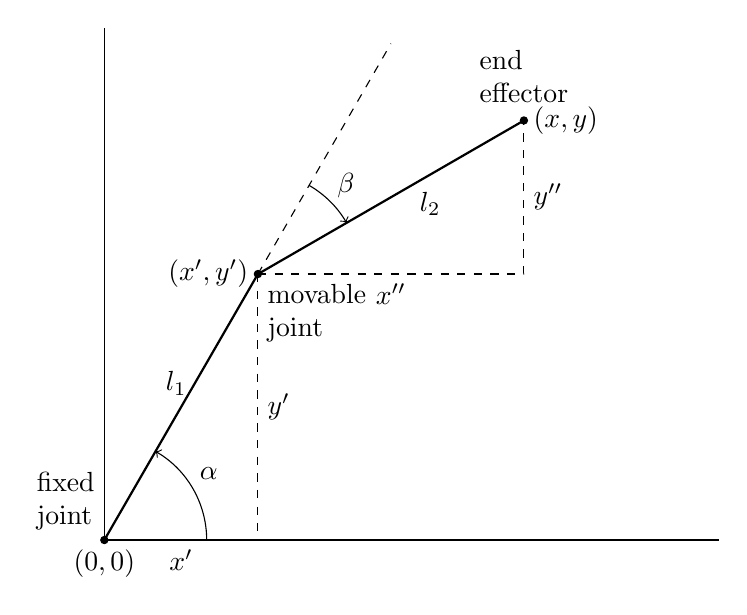
\begin{tikzpicture}[scale=1.3,align=left]
\draw (0,0) coordinate (origin) -- (6,0);
\draw (origin) -- (0,5);
\draw[thick] (origin) -- node[left,xshift=2mm,yshift=3mm] {$l_1$} ++(60:3) coordinate (prime) -- node[below,xshift=5mm,yshift=2mm] {$l_2$} ++(30:3) coordinate (point);
\path (origin) -- ++(60:3) -- ++(30:1) coordinate (angle);
\draw[dashed] (60:3) -- ++(60:2.6);
\draw[->] (1,0) arc (0:60:1) node[midway,xshift=2mm,yshift=2mm] {$\alpha$};
\draw[<-] (angle) arc (30:60:1) node[midway,xshift=2mm,yshift=2mm] {$\beta$};
\draw[fill] (origin) circle [radius=1pt] node[below] {$(0,0)$};
\draw[fill] (prime) circle [radius=1pt] node[left] {$(x',y')$};
\draw[fill] (point) circle [radius=1pt] node[right] {$(x,y)$};
\node[above,yshift=1mm] at (point) {\p{end}\\\p{effector}};
\node[above left] at (origin) {\p{fixed}\\\p{joint}};
\node[below right] at (prime) {\p{movable}\\\p{joint}};
\draw[dashed] (prime) |- (origin);
\draw[dashed] (prime) -| (point);
\path (origin) -- node[below] {$x'$} (prime |- origin);
\path (prime |- origin) -- node[right] {$y'$} (prime);
\path (prime) -- node[below] {$x''$} (prime -| point);
\path (prime -| point) -- node[right] {$y''$} (point);
\end{tikzpicture}
\end{center}
\caption{Forward kinematics of a two-link arm}\label{fig.forward-kinematics}
\end{figure}

Project $(x',y')$ on the $x$- and $y$-axes; by trigonometry its coordinates are:
\begin{eqnarray*}
x' &=& l_1 \cos \alpha\\
y' &=& l_1 \sin \alpha\,.
\end{eqnarray*}
Now take $(x',y')$ as the origin of a new coordinate system and project $(x,y)$ on its axes to obtain $(x'',y'')$. The position of the end effector \emph{relative to} the new coordinate system is:
\begin{eqnarray*}
x'' &=& l_2 \cos (\alpha+\beta)\\
y'' &=& l_2 \sin (\alpha+\beta)\,.
\end{eqnarray*}
In Fig.~\ref{fig.forward-kinematics}, $\beta$ is negative (a clockwise rotation) so $\alpha+\beta$ is the angle between the second link and the line parallel to the $x$-axis.

Combining the results gives:
\begin{eqnarray*}
x &=& l_1 \cos \alpha + l_2 \cos(\alpha + \beta)\\
y &=& l_1 \sin \alpha + l_2 \sin(\alpha + \beta)\,.
\end{eqnarray*}

\noindent\textbf{Example} Let $l_1 = l_2 = 1$, $\alpha = 60^{\circ}$, $\beta = -30^{\circ}$. Then:
\begin{eqnarray*}
x &=& 1\cdot\cos 60 + 1\cdot\cos(60-30) = \frac{1}{2} + \frac{\sqrt{3}}{2} = \frac{1+\sqrt{3}}{2}\\
y &=& 1\cdot\sin 60 + 1\cdot\sin(60-30) = \frac{\sqrt{3}}{2} + \frac{1}{2} = \frac{1+\sqrt{3}}{2}\,.
\end{eqnarray*}

Let us check if this result makes sense. Figure~\ref{fig.kinematics-triangle} shows a triangle formed by adding a line between $(0,0)$ and $(x,y)$. The complement of the angle $\beta$ is $180-30=150$ and the triangle is isoceles since both sides are $1$, so the other angles of the triangle are equal and their values are $(180-150)/2=15$. The angle that the new line forms with the $x$-axis is $60-15=45$, which is consistent with $x=y$.

\begin{figure}
\begin{center}
% Angles of the triangle
\begin{tikzpicture}[scale=1.3]
\draw (0,0) coordinate (origin) node[left] {$(0,0)$} -- (6,0);
\draw (origin) -- ++(60:3) coordinate (prime) -- ++(30:3) coordinate (point);
\path (origin) -- ++(60:3) -- ++(30:1) coordinate (angle);
\draw (origin) -- (point) node[right] {$(x,y)$};
\draw[dashed] (60:3) -- ++(60:2.6);
\draw[fill] (origin) circle [radius=1pt];
\draw[fill] (prime) circle [radius=1pt];
\draw[fill] (point) circle [radius=1pt];
\node[above,xshift=12mm,yshift=8mm] at (prime) {$\beta=30^{\circ}$};
\node[below,xshift=3mm,yshift=0mm] at (prime) {$150^{\circ}$};
\draw[->] (13mm,9mm) -- node[right,xshift=3mm] {$15^{\circ}$} (6mm,9mm);
\draw[->] (41mm,36mm) -- node[right,xshift=3mm] {$15^{\circ}$} (34mm,36mm);
\node[above right,xshift=5mm,yshift=1mm] at (origin) {$\alpha-15^{\circ}=60^{\circ}-15^{\circ}=45^{\circ}$};
\end{tikzpicture}
\end{center}
\caption{Computing the angles}\label{fig.kinematics-triangle}
\end{figure}

\begin{framed}
\act{Forward kinematics}{forward-kinematics}
\begin{itemize}
\item Program your robot so that it traces the path of the arm in Fig.~\ref{fig.forward-kinematics}: turn left $60^{\circ}$, move forward one unit ($1$m or some other convenient distance), turn right $30^{\circ}$, move forward one unit.
\item Measure the $x$- and $y$-distances of the robot from the origin and compare them to the values computed by the equations for forward kinematics.
\end{itemize}
\end{framed}

\section{Inverse kinematics}\label{s.inverse-kinematics}

The gray ring in Fig.~\ref{fig.workspace} shows the \emph{workspace}\index{workspace} of the two-link arm, the set of positions that the end effector can reach. (We assume that $l_2<l_1$.) The workspace is circularly symmetric since we assume that there are no limitations of the rotation of the joints in a full circle between $-180^{\circ}$ and $180^{\circ}$. Any point like $a$ on the circumference of the outer circle is a furthest position of the arm from the origin; it is obtained when the two links are lined up so the arm length is $l_1+l_2$. The closest positions to the origin in the workspace are points like $b$ on the circumference of the inner circle; they are obtained when the second link is bend back on the first link giving a length of $l_1-l_2$. Another reachable position $c$ is shown; there are \emph{two} configurations (rotations of the joints) that cause the arm to be positioned at $c$.

\begin{figure}
\begin{center}
% Workspace of two-level arm
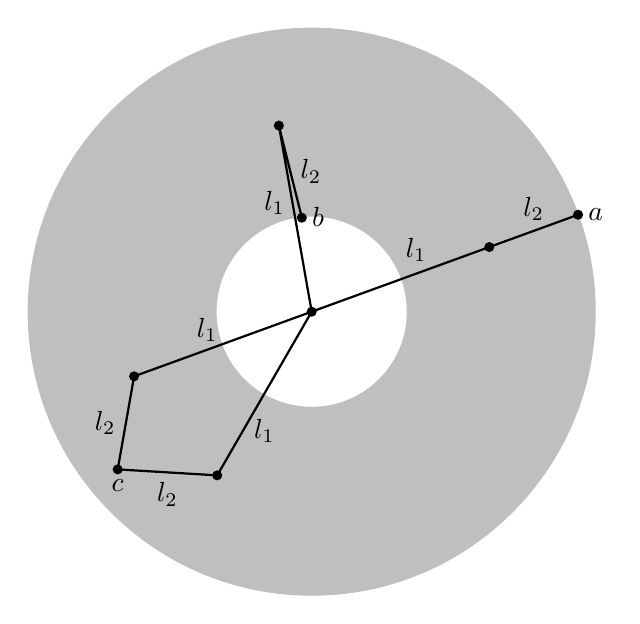
\begin{tikzpicture}[scale=.8]
% Circles
\draw[fill,gray!50] (0,0) coordinate (origin) circle[radius=45mm];
\draw[fill,white] (origin) circle[radius=15mm];
\draw[fill] (origin) circle [radius=2pt];
% First position
\draw[thick] (origin) -- node[above,xshift=2mm,yshift=1mm] {$l_1$} ++(20:30mm) -- node[above] {$l_2$} ++(20:15mm)  node[right] {$a$};
\draw[fill] (20:30mm) circle [radius=2pt];
\draw[fill] (20:45mm) circle [radius=2pt];
% Second position
\draw[thick] (origin) -- node[left,xshift=0mm,yshift=2mm] {$l_1$} ++(100:30mm) -- node[right] {$l_2$} ++(284:15mm)  node[right] {$b$};
\draw[fill] (100:30mm) circle [radius=2pt];
\draw[fill] (96:15mm) circle [radius=2pt];
% Third position
\draw[thick] (origin) -- node[above,xshift=-2mm,yshift=-1mm] {$l_1$} ++(200:30mm) coordinate (mid1) -- node[left] {$l_2$} ++(260:15mm) coordinate (endtwo) node[below] {$c$};
\draw[thick] (origin) -- node[below,,xshift=0mm,yshift=-2mm] {$l_1$} ++(240:30mm) coordinate (mid2) -- node[below] {$l_2$} (endtwo);
\draw[fill] (mid1) circle [radius=2pt];
\draw[fill] (mid2) circle [radius=2pt];
\draw[fill] (endtwo) circle [radius=2pt];
\end{tikzpicture}
\end{center}
\caption{Workspace of a two-lever arm}\label{fig.workspace}
\end{figure}

Under the assumption that $l_2<l_1$, no sequence of rotations can position the end of the arm closer to the origin that $l_1-l_2$ and no position at a distance greater than $l_1+l_2$ from the origin is accessible. From the figure we learn that a problem in inverse kinematics---finding commands to reach a specified point---can have zero, one or many solutions.

The computation of the inverse kinematics uses the \emph{law of cosines} (Fig.~\ref{fig.cosines}):
\[
a^2 + b^2 - 2ab \cos \theta = c^2\,.
\]
In a right triangle $\cos 90^{\circ} = 0$ and the law reduces to the Pythagorean theorem.

\begin{figure}
\begin{center}
% Law of cosines
\begin{tikzpicture}
\draw (0,0) coordinate (origin) --  node[below] {$c$} (6,0) coordinate (two);
\draw (origin) -- node[left] {$a$} ++(60:3) coordinate (one) -- node[above] {$b$} (two);
\node[below,xshift=1mm,yshift=-2mm] at (one) {$\theta$};
\end{tikzpicture}
\end{center}
\caption{Law of cosines}\label{fig.cosines}
\end{figure}

Suppose now that we are given a point $(x,y)$ and we want values for $\alpha,\beta$ (if any exist) which will bring the arm to that point. Figure~\ref{fig.inverse-kinematics} similar to Fig.~\ref{fig.kinematics-triangle} except that the specific values are replaced by arbitrary angles and lengths.

By the Pythagorean theorem, $r=\sqrt{x^2 + y^2}$.

\begin{figure}
\begin{center}
% Inverse kinematics
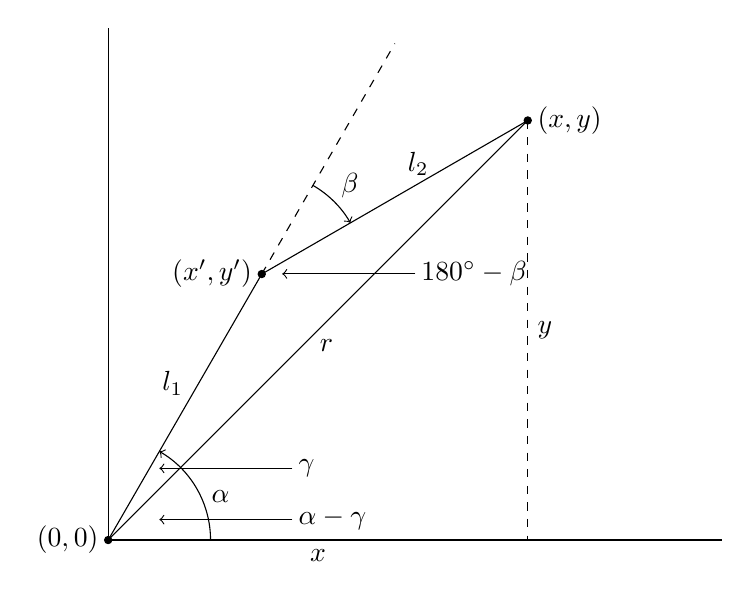
\begin{tikzpicture}[scale=1.3]
\draw (0,0) coordinate (origin) -- (6,0);
\draw (origin) -- (0,5);
\draw (origin) -- node[left,xshift=1mm,yshift=3mm] {$l_1$} ++(60:3) coordinate (prime) -- node[below,xshift=3mm,yshift=7mm] {$l_2$} ++(30:3) coordinate (point);
\draw[dashed] (point) -- node[right] {$y$} (point |- origin);
\draw (origin) -- node[below] {$x$} (origin -| point);
\path (origin) -- ++(60:3) -- ++(30:1) coordinate (angle);
\draw[dashed] (60:3) -- ++(60:2.6);
\draw (origin) -- node[right,xshift=-1mm,yshift=-2mm] {$r$} (point);
\draw[->] (1,0) arc (0:60:1) node[midway,xshift=3mm,yshift=-1mm] {$\alpha$};
\draw[<-] (angle) arc (30:60:1) node[midway,xshift=2mm,yshift=2mm] {$\beta$};
\draw[fill] (origin) circle [radius=1pt] node[left] {$(0,0)$};
\draw[fill] (prime) circle [radius=1pt] node[left] {$(x',y')$};
\draw[fill] (point) circle [radius=1pt] node[right] {$(x,y)$};

\draw[->] (30mm,26mm) -- node[right,xshift=8mm] {$180^{\circ}-\beta$} (17mm,26mm);
\draw[->] (18mm,7mm) -- node[right,xshift=8mm] {$\gamma$} (5mm,7mm);
\draw[->] (18mm,2mm) -- node[right,xshift=8mm] {$\alpha-\gamma$} (5mm,2mm);
\end{tikzpicture}
\end{center}
\caption{Inverse kinematics of a two-link arm}\label{fig.inverse-kinematics}
\end{figure}

The law of cosines gives:
\[
l_1^2 + l_2^2 - 2l_1 l_2 \cos(180^\circ-\beta) = r^2\,,
\]
which can be solved for $\beta$:
\begin{eqnarray*}
\cos(180^\circ-\beta) &=& \frac{l_1^2 + l_2^2 - r^2}{2l_1 l_2}\\
\beta &=& 180^\circ-\cos^{-1}\left(\frac{l_1^2 + l_2^2 - r^2}{2l_1 l_2}\right)\,.
\end{eqnarray*}
To obtain $\gamma$ and then $\alpha$, use the law of cosines with $\gamma$ as the central angle:
\[
\cos\gamma = \frac{l_1^2 +r^2 - l_2^2}{2l_1 r}\,.
\]
From the right triangle formed by $(x,y)$ we have:
\begin{eqnarray*}
\tan(\alpha - \gamma) &=& \frac{y}{x}\\
\alpha &=& \tan^{-1} \frac{y}{x} + \gamma\,,
\end{eqnarray*}
so:
\[
\alpha = \tan^{-1} \frac{y}{x} + \cos^{-1}\left(\frac{l_1^2 +r^2 - l_2^2}{2l_1 r}\right)\,.
\]

\noindent\textbf{Example} Assume again that $l_1 = l_2 = 1$ and that the end effector is at the point computed from the forward kinematics:
\[
(x,y) = \left(\frac{1+\sqrt{3}}{2},\frac{1+\sqrt{3}}{2}\right)\,.
\]
First, compute $r^2$:
\[
r^2 = x^2+y^2 = \left( \frac{1+\sqrt{3}}{2}\right)^2 + \left( \frac{1+\sqrt{3}}{2}\right)^2 = 2+\sqrt{3}\,,
\]
and use it in the computation of $\beta$:
\begin{eqnarray*}
\beta &=& 180^{\circ} - \cos^{-1} \left(\frac{1^2 + 1^2 - (2+\sqrt{3})}{2\cdot 1\cdot 1}\right)\\
&=& 180^{\circ} - \cos^{-1}\left(-\frac{\sqrt{3}}{2}\right)\\
&=& 180^{\circ} \pm 150^{\circ}\\
&=& \pm 30^{\circ}\,,
\end{eqnarray*}
since $330^{\circ}=-30^{\circ} \!\!\!\pmod{360^\circ}$. There are two solutions because there are two ways of moving the arm to $(x,y)$.

Next compute $\gamma$:
\begin{equation}
\gamma = \cos^{-1}\left(\frac{1^2 + r^2 - 1^2}{2\cdot 1 \cdot r}\right) = \cos^{-1}\left(\frac{r}{2}\right)= \cos^{-1}\left(\frac{\sqrt{2+\sqrt{3}}}{2}\right) = \pm 15^{\circ}\,.\label{eq.cos15}
\end{equation}
The inverse cosine can be obtained numerically on a calculator or algebraically as shown in Appendix~\ref{a.cosine}.

Since $x=y$, the computation of $\alpha$ is easy:
\[\alpha = \tan^{-1}\frac{y}{x} + \gamma = \tan^{-1}1 + \gamma = 45^{\circ} \pm 15^{\circ} = 60^{\circ} \;\textrm{or}\; 30^{\circ}\,.
\]
The solution $\alpha=60^{\circ},\beta=-30^{\circ}$ corresponds to the rotation of the joints in Fig.~\ref{fig.forward-kinematics}, while the solution $\alpha=30^{\circ},\beta=30^{\circ}$ corresponds to rotating both of the joints $30^{\circ}$ counterclockwise.

In this simple case, it is possible to solve the forward kinematics equation to obtain formulas for the inverse kinematics. In general this is not possible so approximate numerical solutions are used.

\begin{framed}
\act{Inverse kinematics}{inverse-kinematics}
\begin{itemize}
\item Use the formulas for the inverse kinematics to program your robot to move to a specified coordinate.
\item Measure the $x$- and $y$-distances of the robot from the origin and compare them to the specified coordinates.
\item If your robot's computer does not have the capability to compute the formulas, compute them offline and then input the commands to the robot.
\end{itemize}
\end{framed}

%%%%%%%%%%%%%%%%%%%%%%%%%%%%%%%%%%%%%%%%%%%%%%%%%%%%%%%%%%%

\section{Rotations}\label{s.rotations}
\index{rotation}

The motion of a robotic manipulator is described in terms of \emph{coordinate frames}\index{coordinate frame}. Three frames are associated with the arm in Fig.~\ref{fig.forward-kinematics}: one frame is associated with the joint at the origin (which we assume is fixed to a table or the floor), a second frame is associated with the joint between the two links,  and a third frame is associated with the end effector at the end of the second link.

In this section we describe how the rotational motion of a robotic arm can be mathematically modeled using \emph{rotation matrices}. The links in robotic arms introduce \emph{translations}: the second joint is offset by a linear distance of $l_1$ from the first joint, and the end effector is offset by a linear distance of $l_2$ from the second joint. The mathematical treatment of translations uses an extension of rotation matrices called \emph{homogeneous transforms}.

Rotations can be confusing because a rotation matrix can have three interpretations that are described in the following subsections: rotating a vector, rotating a coordinate frame and transforming a vector from one coordinate frame to another.

\subsection{Rotating a vector}
\index{rotation!vector@of a vector}

Consider a vector with cartesian coordinates $(x,y)$ and polar coordinates $(r,\phi)$ (Fig.~\ref{fig.one-vector}). Now rotate the vector by an angle $\theta$ (Fig.~\ref{fig.rotated-vector}). Its polar coordinates are $(r,\phi+\theta)$. What are its cartesian coordinates?

\begin{figure}
\subfigures
\begin{minipage}{\textwidth}
\leftfigure{
\begin{tikzpicture}[scale=1.3]
\draw (0,0) coordinate (origin) -- (4,0);
\draw (origin) -- (0,3);
\path[->] (origin) -- ++(30:3.5) coordinate (point);
\draw[->] (origin) -- node[above] {$r$} ++(30:3.46);
\draw[fill] (point) circle [radius=1pt];
\draw (point) -- node[right] {$y$} (point |- origin);
\draw (origin) -- node[below,xshift=2mm] {$x$} (point |- origin);
\draw (1,0) arc (0:30:1) node[midway,xshift=3mm] {$\phi$};
\draw[fill] (origin) circle [radius=1pt];
\end{tikzpicture}
}
\hspace{\fill}
\rightfigure{
\begin{tikzpicture}[scale=1.3]
\draw (0,0) coordinate (origin) -- (4,0);
\draw (origin) -- (0,3);
\path[->] (origin) -- ++(60:3.5) coordinate (point);
\draw[->] (origin) -- node[above] {$r$} ++(60:3.46);
\draw[fill] (point) circle [radius=1pt];
\draw (point) -- node[right] {$y'$} (point |- origin);
\draw (origin) -- node[below,xshift=2mm] {$x'$} (point |- origin);
\draw (1,0) arc (0:60:1);
\node at (1.2,.7) {$\phi+\theta$};
\draw[fill] (origin) circle [radius=1pt];
\end{tikzpicture}
}
\leftcaption{A vector}\label{fig.one-vector}
\rightcaption{The vector rotated by $\theta$}\label{fig.rotated-vector}
\end{minipage}
\end{figure}

Using the trigonometric identities for the sum of two angles and the conversion of $(r,\phi)$ to $(x,y)$ we have:
\begin{eqnarray*}
x' &=& r\cos(\phi+\theta)\\
&=&r\cos\phi\cos\theta - r\sin\phi\sin\theta\\
&=&(r\cos\phi)\cos\theta - (r\sin\phi)\sin\theta\\
&=&x\cos\theta - y\sin\theta\,,\\
\\
y' &=& r\sin(\phi+\theta)\\
&=&r\sin\phi\cos\theta + r\cos\phi\sin\theta\\
&=&(r\sin\phi)\cos\theta + (r\cos\phi)\sin\theta\\
&=&y\cos\theta + x\sin\theta\\
&=&x\sin\theta + y\cos\theta\,.\\
\end{eqnarray*}
These equations can be expressed as the multiplication of a matrix called the \emph{rotation matrix}\index{rotation!matrix!two-dimensional} and a vector:
\[
\spacearray
\left[\begin{array}{c}x'\\y'\end{array}\right]=
\left[\begin{array}{cc}\cos\theta&-\sin\theta\\\sin\theta&\cos\theta\end{array}\right]
\left[\begin{array}{c}x\\y\end{array}\right]\,.
\]

\medskip

\noindent\textbf{Example} Let $p$ be the point at the tip of a vector of length $r=1$ that forms an angle of $\phi=30^{\circ}$ with the positive $x$-axis. The cartesian coordinates of $p$ are $\left(\frac{\sqrt{3}}{2},\,\frac{1}{2}\right)$. Suppose that the vector is rotated by $\theta=30^{\circ}$. What are the new cartesian coordinates of $p$? Using matrix multiplication:
\[
\spacearray
\left[\begin{array}{c}x'\\y'\end{array}\right]\;=\;
\left[\begin{array}{cc}\frac{\sqrt{3}}{2}&-\frac{1}{2}\\\frac{1}{2}&\frac{\sqrt{3}}{2}\end{array}\right]
\left[\begin{array}{c}\frac{\sqrt{3}}{2}\\\frac{1}{2}\end{array}\right]\;=\;
\left[\begin{array}{c}\frac{1}{2}\\\frac{\sqrt{3}}{2}\end{array}\right]\,.
\]
The result makes sense because rotating a vector whose angle with the $x$-axis is $30^{\circ}$ by $30^{\circ}$ should give a vector whose angle with the $x$-axis is $60^{\circ}$.

Suppose that the vector is rotated by an additional $30^{\circ}$; its new coordinates are:
\begin{equation}\label{eq.rotate1}
\spacearray
\left[\begin{array}{cc}\frac{\sqrt{3}}{2}&-\frac{1}{2}\\\frac{1}{2}&\frac{\sqrt{3}}{2}\end{array}\right]\;\;
\left(\left[\begin{array}{cc}\frac{\sqrt{3}}{2}&-\frac{1}{2}\\\frac{1}{2}&\frac{\sqrt{3}}{2}\end{array}\right]
\left[\begin{array}{c}\frac{\sqrt{3}}{2}\\\frac{1}{2}\end{array}\right]\right)\;=\;
\left[\begin{array}{cc}\frac{\sqrt{3}}{2}&-\frac{1}{2}\\\frac{1}{2}&\frac{\sqrt{3}}{2}\end{array}\right]
\left[\begin{array}{c}\frac{1}{2}\\\frac{\sqrt{3}}{2}\end{array}\right]\;=\;
\left[\begin{array}{c}0\\1\end{array}\right]\,.
\end{equation}
This result also makes sense. Rotating a vector whose angle is $30^{\circ}$ twice by $30^{\circ}$ (for a total of $60^\circ$) should give $90^{\circ}$. The cosine of $90^{\circ}$ is $0$ and the sine of $90^{\circ}$ is $1$.

Since matrix multiplication is associative, the multiplication could also be performed as follows:
\begin{equation}\label{eq.rotate2}
\spacearray
\left(\left[\begin{array}{cc}\frac{\sqrt{3}}{2}&-\frac{1}{2}\\\frac{1}{2}&\frac{\sqrt{3}}{2}\end{array}\right]
\left[\begin{array}{cc}\frac{\sqrt{3}}{2}&-\frac{1}{2}\\\frac{1}{2}&\frac{\sqrt{3}}{2}\end{array}\right]\right)\;\;
\left[\begin{array}{c}\frac{\sqrt{3}}{2}\\\frac{1}{2}\end{array}\right]\,.
\end{equation}

\begin{framed}
\act{Rotation matrices}{rotation-matrix}
\begin{itemize}
\item Demonstrate the associativity of matrix multiplication by showing that the multiplication in Eq.~\ref{eq.rotate2} gives the same result as the multiplication in Eq.~\ref{eq.rotate1}.
\item Compute the matrix for a rotation of $-30^{\circ}$ and show that multiplying this matrix by the matrix for a rotation of $30^{\circ}$ gives the matrix for a rotation of $0^{\circ}$.
\item Is this multiplication commutative?
\item Is multiplication of two-dimensional rotational matrices commutative?
\end{itemize}
\end{framed}

\subsection{Rotating a coordinate frame}
\index{rotation!coordinate@of a coordinate frame}

Let us reinterpret Figs.~\ref{fig.one-vector}--\ref{fig.rotated-vector}. Figure~\ref{fig.one-frame} shows a coordinate frame (blue) defined by two orthogonal unit vectors:
\[
\vec{x}= \left[\begin{array}{c}1\\0\end{array}\right]\,,\;\;
\vec{y}= \left[\begin{array}{c}0\\1\end{array}\right]\,.
\]
Fig.~\ref{fig.frame-rotated} shows the \emph{coordinate frame} rotated by $\theta$ degrees (red). The new unit vectors $\vec{x'}$ and $\vec{y'}$ can be obtained by multiplication by the rotation matrix derived above:
\begin{eqnarray*}
\vec{x'}&=&
\left[\spacearray\begin{array}{cc}\cos\theta&-\sin\theta\\\sin\theta&\cos\theta\end{array}\right]
\left[\spacearray\begin{array}{c}1\\0\end{array}\right]=
\left[\spacearray\begin{array}{l}\cos \theta\\\sin\theta\;\;\:\end{array}\right]\\
\,\\
\vec{y'}&=&
\left[\spacearray\begin{array}{cc}\cos\theta&-\sin\theta\\\sin\theta&\cos\theta\end{array}\right]
\left[\spacearray\begin{array}{c}0\\1\end{array}\right]=
\left[\spacearray\begin{array}{l}-\sin \theta\\\cos\theta\end{array}\right]\,.
\end{eqnarray*}

\begin{figure}
\subfigures
\begin{minipage}{\textwidth}
\leftfigure{
\begin{tikzpicture}[scale=1.3]
\draw (0,0) coordinate (origin) -- (3.4,0);
\draw (origin) -- (0,2.8);
\draw[->,thick,blue] (0,0) -- node[below] {$\vec{x}$} (2,0);
\draw[->,thick,blue] (0,0) -- node[left] {$\vec{y}$} (0,2);
\end{tikzpicture}
}
\hspace{\fill}
\rightfigure{
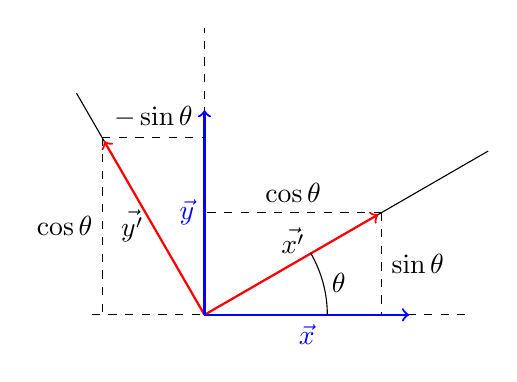
\begin{tikzpicture}[scale=1.3]
\begin{scope}[rotate=30]
\draw (0,0) coordinate (origin) -- (3.2,0);
\draw (origin) -- (0,2.5);
\path (0,0) -- node[above] {$\vec{x'}$} (2,0) coordinate (xprime);
\path (0,0) -- node[left] {$\vec{y'}$} (0,2) coordinate (yprime);
\draw[->,thick,red] (0,0) -- (1.96,0);
\draw[->,thick,red] (0,0) -- (0,1.96);
\end{scope}
\draw[dashed] (-1.1,0) -- (origin) -- (2.6,0);
\draw[dashed] (origin) -- (0,2.8);
\draw[->,thick,blue] (0,0) -- node[below] {$\vec{x}$} (2,0);
\draw[->,thick,blue] (0,0) -- node[left] {$\vec{y}$} (0,2);
\draw[dashed] (xprime) -- node[right] {$\sin \theta$} (xprime |- origin);
\draw[dashed] (xprime) -- node[above] {$\cos \theta$} (origin |- xprime);
\draw[dashed] (yprime) -- node[left] {$\cos \theta$} (yprime |- origin);
\draw[dashed] (yprime) -- node[above] {$-\sin \theta$} (origin |- yprime);
\draw (1.2,0) arc (0:30:1.2) node[midway,xshift=2mm,yshift=0mm] {$\theta$};
\end{tikzpicture}
}
\leftcaption{Original coordinate frame (blue)}\label{fig.one-frame}
\rightcaption{New coordinate frame (red) obtained by rotating the original coordinate frame (blue) by $\theta$}\label{fig.frame-rotated}
\end{minipage}
\end{figure}

\medskip

\noindent\textbf{Example} For the unit vectors in Fig.~\ref{fig.one-frame} and a rotation of $30^\circ$:
\begin{eqnarray*}
\vec{x'}&=&\left[\spacearray\begin{array}{cc}\frac{\sqrt{3}}{2}&-\frac{1}{2}\\\frac{1}{2}&\frac{\sqrt{3}}{2}\end{array}\right]
\left[\spacearray\begin{array}{c}1\\0\end{array}\right]=
\left[\spacearray\begin{array}{c}\frac{\sqrt{3}}{2}\\\frac{1}{2}\end{array}\right]\\
\,\\
\vec{y'}&=&\left[\spacearray\begin{array}{cc}\frac{\sqrt{3}}{2}&-\frac{1}{2}\\\frac{1}{2}&\frac{\sqrt{3}}{2}\end{array}\right]
\left[\spacearray\begin{array}{c}0\\1\end{array}\right]=
\left[\spacearray\begin{array}{c}-\frac{1}{2}\\\frac{\sqrt{3}}{2}\end{array}\right]\,.
\end{eqnarray*}

\subsection{Transforming a vector from one coordinate frame to another}
\index{rotation!transforming a vector from one coordinate frame to another}

Let the origin of a coordinate frame $b$ (blue) represent the joint of an end effector such as a welder and let point $p$ be the tip of the welder (Fig.~\ref{fig.frameb}). By convention in robotics, the coordinate frame of an entity is denoted by a ``pre'' superscript.\footnote{The convention is to use uppercase letters for both the frame and the coordinates, but we use lowercase for clarity.}  In the frame $b$, the point $\bp$ has polar coordinates $(r,\phi)$ and cartesian coordinates $(\bx,\by)$ related by the usual trigonometric formulas:
\[
\bp = (\bx,\by) = (r\cos\phi,\, r\sin\phi)\,.
\]

\begin{figure}
\subfigures
\begin{minipage}{\textwidth}
\leftfigure{
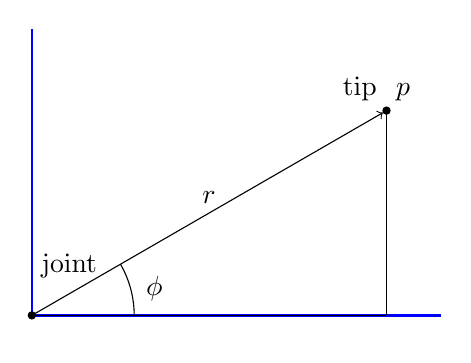
\begin{tikzpicture}[scale=1.3]
\draw[thick,blue] (0,0) coordinate (origin) -- (4,0);
\draw[thick,blue] (origin) -- (0,2.8);
\path (origin) -- node[above] {$r$} ++(30:4) coordinate (point) node[above right] {$p$};
\draw[->] (origin) -- ++(30:3.96);
\draw[fill] (point) circle [radius=1pt] node[above left] {\p{tip}};
\draw (point) -- node[right] {$\by$} (point |- origin);
\draw (origin) -- node[below,xshift=2mm] {$\bx$} (point |- origin);
\draw (1,0) arc (0:30:1) node[midway,xshift=3mm] {$\phi$};
\draw[fill] (origin) circle [radius=1pt] node[above right,yshift=10pt] {\p{joint}};
\end{tikzpicture}
}
\hspace{\fill}
\rightfigure{
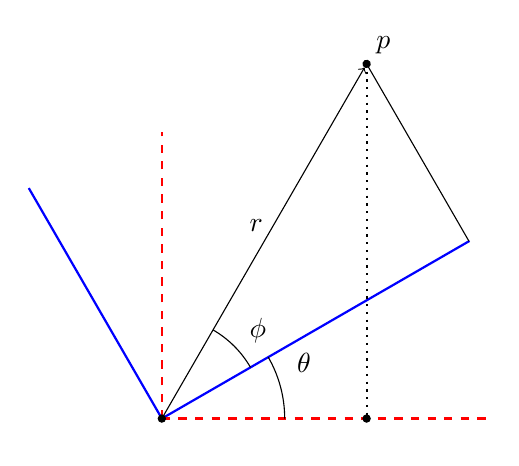
\begin{tikzpicture}[scale=1.3]
\begin{scope}[rotate=30]
\draw[thick,blue] (0,0) coordinate (origin) -- node[black,below,xshift=12mm,yshift=6mm] {$\bx$} (3.47,0);
\draw[thick,blue] (origin) -- (0,2.6);
\path (origin) -- node[above,xshift=-1mm] {$r$} ++(30:4) coordinate (point) node[above right] {$p$};
\draw[->] (origin) -- ++(30:3.96);
\draw[fill] (point) circle [radius=1pt];
\draw (point) -- node[right] {$\by$} (point |- origin);
\draw (1,0) arc (0:30:1) node[midway,xshift=3mm,yshift=2mm] {$\phi$};
\end{scope}
\draw[thick,dashed,red] (origin) -- (3.2,0);
\draw[thick,dashed,red] (origin) -- (0,2.8);
\draw[thick,dotted] (point) -- node[right] {$\ay$} (point |- origin);
\draw[fill] (point |- origin) circle [radius=1pt];
\path[dashed] (origin) -- node[below,xshift=2mm] {$\ax$} (point |- origin);
\draw (1.2,0) arc (0:30:1.2) node[midway,xshift=3mm,yshift=3mm] {$\theta$};
\draw[fill] (origin) circle [radius=1pt];
\end{tikzpicture}
}
\leftcaption{Point $p$ at the tip of an end effector in coordinate frame $b$ (blue)}\label{fig.frameb}
\rightcaption{Point $p$ in coordinate frames $a$ (red) and $b$ (blue)}\label{fig.framea}
\end{minipage}
\end{figure}

Suppose that the joint (\emph{with its coordinate frame}) is rotated by the angle $\theta$. The coordinates of the point relative to $b$ remain the same, but the coordinate frame has moved so we ask: What are the coordinates $\ap=(\ax,\ay)$ of the point in the coordinate frame before it was moved? In Fig.~\ref{fig.framea} the original frame $b$ is shown rotated to a new position (and still shown in blue), while the coordinate frame $a$ is in the old position of $b$ and is shown as red dashed lines. In the previous section we asked how to transform one coordinate frame into another; here, we are asking how to transform the coordinates of a point in a frame to its coordinates in another frame.

In terms of the robotic arm: we know $(\bx,\by)$, the coordinates of the tip of the end effector relative to the frame of the end effector, and we now ask for its coordinates $\ap=(\ax,\ay)$ relative to the fixed base. This is important because if we know $\ap$, we can compute the distance and angle from the tip of the welder to the parts of the car it must now weld.

We can repeat the computation used for rotating a vector:
\begin{eqnarray*}
\ax &=& r\cos(\phi+\theta)\\
&=&r\cos\phi\cos\theta - r\sin\phi\sin\theta\\
&=&\bx\cos\theta - \by\sin\theta\,,\\
\\
\ay &=& r\sin(\phi+\theta)\\
&=&r\sin\phi\cos\theta + r\cos\phi\sin\theta\\
&=&\bx\sin\theta + \by\cos\theta\,,\\
\end{eqnarray*}
to obtain the rotation matrix:
\begin{equation}
\spacearray
\left[\begin{array}{c}\ax\\\ay\end{array}\right]=
\left[\begin{array}{cc}\cos\theta&-\sin\theta\\\sin\theta&\cos\theta\end{array}\right]
\left[\begin{array}{c}\bx\\\by\end{array}\right]\,.\label{eq.frame-to-frame}
\end{equation}
The matrix is called the rotation matrix \emph{from} frame $b$ \emph{to} frame $a$ and denoted $\leftidx{^a_b}{R}{}$. Pre-multiplying the point $\bp$ in frame $b$ by the rotation matrix gives $\ap$ its coordinates in frame $a$:
\[
\ap = \leftidx{^a_b}{R}{} \; \bp\,.
\]

\medskip

\noindent\textbf{Example} Let $\bp$ be the point in frame $b$ at the tip of a vector of length $r=1$ that forms an angle of $\phi=30^{\circ}$ with the positive $x$-axis. The coordinates of $\bp$ are $\left(\frac{\sqrt{3}}{2},\,\frac{1}{2}\right)$. Suppose that the coordinate frame $b$ (together with the point $p$) is rotated by $\theta=30^{\circ}$ to obtain the coordinate frame $a$. What are the coordinates of $\ap$? Using Eq.~\ref{eq.frame-to-frame}:
\[
\spacearray
\ap=
\left[\begin{array}{c}\ax\\\ay\end{array}\right]\;=\;
\left[\begin{array}{cc}\frac{\sqrt{3}}{2}&-\frac{1}{2}\\\frac{1}{2}&\frac{\sqrt{3}}{2}\end{array}\right]
\left[\begin{array}{c}\frac{\sqrt{3}}{2}\\\frac{1}{2}\end{array}\right]\;=\;
\left[\begin{array}{c}\frac{1}{2}\\\frac{\sqrt{3}}{2}\end{array}\right]\,.
\]
If frame $a$ is now rotated $30^{\circ}$, we obtain the coordinates of the point in a third frame $a1$. Pre-multiply $\ap$ by the rotation matrix for $30^{\circ}$ to obtain $\aprimep$:
\[
\spacearray
\aprimep = \left[\begin{array}{cc}\frac{\sqrt{3}}{2}&-\frac{1}{2}\\\frac{1}{2}&\frac{\sqrt{3}}{2}\end{array}\right]\;\;
\left(\left[\begin{array}{cc}\frac{\sqrt{3}}{2}&-\frac{1}{2}\\\frac{1}{2}&\frac{\sqrt{3}}{2}\end{array}\right]
\left[\begin{array}{c}\frac{\sqrt{3}}{2}\\\frac{1}{2}\end{array}\right]\right)\;=\;
\left[\begin{array}{cc}\frac{\sqrt{3}}{2}&-\frac{1}{2}\\\frac{1}{2}&\frac{\sqrt{3}}{2}\end{array}\right]
\left[\begin{array}{c}\frac{1}{2}\\\frac{\sqrt{3}}{2}\end{array}\right]\;=\;
\left[\begin{array}{c}0\\1\end{array}\right]\,.
\]
The product of the two rotation matrices:
\[
\spacearray
\left[\begin{array}{cc}\frac{\sqrt{3}}{2}&-\frac{1}{2}\\\frac{1}{2}&\frac{\sqrt{3}}{2}\end{array}\right]
\left[\begin{array}{cc}\frac{\sqrt{3}}{2}&-\frac{1}{2}\\\frac{1}{2}&\frac{\sqrt{3}}{2}\end{array}\right]=
\left[\begin{array}{cc}\frac{1}{2}&-\frac{\sqrt{3}}{2}\\\frac{\sqrt{3}}{2}&\frac{1}{2}\end{array}\right]
\]
results in the rotation matrix for rotating the original coordinate frame $b$ by $60^{\circ}$:
\[
\spacearray
\left[\begin{array}{cc}\frac{1}{2}&-\frac{\sqrt{3}}{2}\\\frac{\sqrt{3}}{2}&\frac{1}{2}\end{array}\right]
\left[\begin{array}{c}\frac{\sqrt{3}}{2}\\\frac{1}{2}\end{array}\right]\;=\;
\left[\begin{array}{c}0\\1\end{array}\right]\,.
\]

Given a sequence of rotations, pre-multiplying their rotation matrices gives the rotation matrix for the rotation equivalent to the sum of the individual rotations.

\section{Rotating and translating a coordinate frame}\label{s.rotate-translate}

The joints on robotics manipulators are connected by links so the coordinate systems are related not just by rotations but also by translations. The point $p$ in Fig.~\ref{fig.before-rotate} represents a point in the (red) coordinate frame $b$, but relative to the (blue dashed) coordinate frame $a$, frame $b$ is both rotated by the angle $\theta$ and its origin is translated by $\Delta x$ and $\Delta y$. If $\bp=(\bx,\by)$, the coordinates of the point in frame $b$, are known, what are its coordinates $\ap=(\ax,\ay)$ in frame $a$?

\begin{figure}
\begin{center}
\begin{tikzpicture}[scale=1.3]
\begin{scope}[yshift=1cm,xshift=3cm,rotate around={30:(0,0)}]
\draw[thick,red] (0,0) coordinate (origin) -- node[black,near end,xshift=8mm,yshift=-2mm] {\p{frame b}} (4,0);
\draw[thick,red] (origin) -- (0,3);
\path (origin) -- node[above,xshift=-1mm] {$r$} ++(30:4) coordinate (point) node[above right] {$p$};
\draw[->] (origin) -- ++(30:3.96);
\draw[fill] (point) circle [radius=1pt];
\draw (point) -- node[right] {$\by$} (point |- origin);
\path (origin) -- node[below,xshift=5mm,yshift=2mm] {$\bx$} (point |- origin);
\draw (1,0) arc (0:30:1) node[midway,xshift=3mm,yshift=2mm] {$\phi$};
\end{scope}
\draw[dashed,thick,blue] (0,0) coordinate (origina) -- node[black,below,midway,yshift=-1mm] {\p{frame a}} (6,0);
\draw[dashed,thick,blue] (origina) -- (0,3);
\draw[->] (origina) -- ($ (origina) ! .985 ! (point) $);
\draw[dashed] (origin) -- (point |- origin);
\draw (4.5,1) arc (0:30:1.45) node[midway,xshift=2mm] {$\theta$};
\draw[dotted,thick] (origin) -- (origin |- origina) node [right,midway] {$\Delta y$};
\draw[dotted,thick] (origin) -- (origina |- origin) node [below,midway] {$\Delta x$};
\draw[fill] (origin) circle [radius=1pt];
\draw[fill] (origina) circle [radius=1pt];
\end{tikzpicture}
\caption{Frame $b$ is rotated and translated to frame $a$}\label{fig.before-rotate}
\end{center}
\end{figure}

To perform this computation, we define an intermediate (green) coordinate frame $a1$ that has the same origin as $b$ and the same orientation as $a$ (Fig.~\ref{fig.after-rotate}). What are the coordinates $\aprimep=(\aprimex,\aprimey)$ of the point in frame $a1$? This is simply the rotation by $\theta$ that we have done before:
\[
\spacearray
\aprimep=\left[\begin{array}{c}\aprimex\\\aprimey\end{array}\right]=
\left[\begin{array}{cc}\cos\theta&-\sin\theta\\\sin\theta&\cos\theta\end{array}\right]
\left[\begin{array}{c}\bx\\\by\end{array}\right]\,.
\]
Now that we have the coordinates of the point in $a1$, it is easy to obtain the coordinates in frame $a$ by adding the offsets of the translation. In matrix form:
\[
\spacearray
\ap=\left[\begin{array}{c}\ax\\\ay\end{array}\right]=
\left[\begin{array}{c}\aprimex\\\aprimey\end{array}\right]\,+\,
\left[\begin{array}{c}\Delta x\\\Delta y\end{array}\right]\,.
\]

\begin{figure}
\begin{center}
\begin{tikzpicture}[scale=1.3]
\begin{scope}[yshift=1cm,xshift=3cm,rotate around={30:(0,0)}]
\draw[thick,red] (0,0) coordinate (origin) -- node[black,near end,xshift=8mm,yshift=-2mm] {\p{frame b}} (4,0);
\draw[thick,red] (origin) -- (0,3);
\path (origin) -- ++(30:4) coordinate (point) node[above right] {$p$};
\draw[->] (origin) -- ++(30:3.96);
\draw[fill] (point) circle [radius=1pt];
\draw (1,0) arc (0:30:1) node[midway,xshift=3mm,yshift=2mm] {$\phi$};
\end{scope}
\draw[thick,green!60!black] (origin) -- node[black,below,midway,xshift=4mm] {\p{frame a1}} +(4,0);
\draw[thick,green!60!black] (origin) -- +(0,4);
\draw[dotted,thick] (point) -- node [right,midway] {$\aprimey$} (point |- origin);
\draw[dotted,thick] (point) -- node [above,midway] {$\aprimex$} (origin |- point);
\draw[dashed,thick,blue] (0,0) coordinate (origina) -- node[black,below,midway,yshift=-1mm] {\p{frame a}} (6,0);
\draw[dashed,thick,blue] (origina) -- (0,3);
\draw[->] (origina) -- ($ (origina) ! .985 ! (point) $);
\draw (4.5,1) arc (0:30:1.45) node[midway,xshift=2mm] {$\theta$};
\draw[dotted,thick] (origin) -- (origin |- origina) node [right,midway] {$\Delta y$};
\draw[dotted,thick] (origin) -- (origina |- origin) node [below,midway] {$\Delta x$};
\draw[fill] (origin) circle [radius=1pt];
\draw[fill] (origina) circle [radius=1pt];
\end{tikzpicture}
\caption{Frame $b$ is rotated to frame $a1$ and then translated to frame $a$}\label{fig.after-rotate}
\end{center}
\end{figure}

\emph{Homogeneous transforms}\index{homogeneous transform} are used to combine a rotation and a translation in one operator. The two-dimensional vector giving the coordinates of a point is extended with a third element that has a fixed value of $1$:
\[
\spacearray
\left[\begin{array}{c}x\\y\\1\end{array}\right]\,.
\]
The rotation matrix is extended to a $3\times 3$ matrix with a $1$ in the lower right corner and zeros elsewhere. It is easy to check that multiplication of a vector in frame $b$ by the rotation matrix results in the same vector as before except for the extra $1$ element:
\[
\spacearray
\left[\begin{array}{c}\leftidx{^{a1}}\!{x}{}\\\leftidx{^{a1}}\!{y}{}\\1\end{array}\right]\;=\;
\left[\begin{array}{ccc}\cos\theta&-\sin\theta&0\\\sin\theta&\cos\theta&0\\0&0&1\end{array}\right]
\left[\begin{array}{c}\bx\\\by\\1\end{array}\right]\,.
\]
The result is the coordinates of the point in the intermediate frame $a1$. To obtain the coordinates in frame $a$, we multiply by a matrix that performs the translation:
\[
\spacearray
\left[\begin{array}{c}\ax\\\ay\\1\end{array}\right]\;=\;
\left[\begin{array}{ccc}1&0&\Delta x\\0&1&\Delta y\\0&0&1\end{array}\right]
\left[\begin{array}{c}\leftidx{^{a1}}\!{x}{}\\\leftidx{^{a1}}\!{y}{}\\1\end{array}\right]\,.
\]
By multiplying the two transforms, we obtain a single homogeneous transform that can perform both the rotation and that translation:
\[
\spacearray
\left[\begin{array}{ccc}1&0&\Delta x\\0&1&\Delta y\\0&0&1\end{array}\right]
\left[\begin{array}{ccc}\cos\theta&-\sin\theta&0\\\sin\theta&\cos\theta&0\\0&0&1\end{array}\right]\;=\;
\left[\begin{array}{ccc}\cos\theta&-\sin\theta&\Delta x\\\sin\theta&\cos\theta&\Delta y\\0&0&1\end{array}\right]\,.
\]

\noindent\textbf{Example} Let us extend the previous example by adding a translation of $(3,1)$ to the rotation of $30^\circ$. The homogeneous transform of the rotation followed by the translation is:
\[
\spacearray
\left[\begin{array}{ccc}1&0&3\\0&1&1\\0&0&1\end{array}\right]
\left[\begin{array}{ccc}\frac{\sqrt{3}}{2}&-\frac{1}{2}&0\\\frac{1}{2}&\frac{\sqrt{3}}{2}&0\\0&0&1\end{array}\right]\;\;=
\left[\begin{array}{ccc}\frac{\sqrt{3}}{2}&-\frac{1}{2}&3\\\frac{1}{2}&\frac{\sqrt{3}}{2}&1\\0&0&1\end{array}\right]\,.
\]
The coordinates of the point in frame $a$ are:
\[
\spacearray
\left[\begin{array}{c}\ax\\\ay\\1\end{array}\right]\;=\;
\left[\begin{array}{ccc}\frac{\sqrt{3}}{2}&-\frac{1}{2}&3\\\frac{1}{2}&\frac{\sqrt{3}}{2}&1\\0&0&1\end{array}\right]
\left[\begin{array}{c}\frac{\sqrt{3}}{2}\\\frac{1}{2}\\1\end{array}\right]\;=\;
\left[\begin{array}{c}\frac{1}{2}+3\\\frac{\sqrt{3}}{2}+1\\1\end{array}\right]\,.
\]

\begin{framed}
\act{Homogeneous transforms}{homogeneous}

\begin{itemize}
\item Draw the diagram for a rotation of $-30^\circ$ followed by a translation of $(3,-1)$.
\item Compute the homogeneous transform.
\end{itemize}
\end{framed}

%%%%%%%%%%%%%%%%%%%%%%%%%%%%%%%%%%%%%%%%%%%%%%%%%%%%%%%%%%%

\section{A taste of three-dimensional rotations}\label{s.three}

\index{rotation!three-dimensional}

The concepts of coordinate transformations and kinematics in three-dimensions are the same as in two dimensions, however, the mathematics is more complicated. Furthermore, many of us find it difficult to visualize three-dimensional motion when all we are shown are two-dimensional representations of three-dimensional objects. In this section we give a taste of three-dimensional robotics by looking at rotations in three dimensions.

\subsection{Rotations around the three axes}\label{s.rotation-notation}

A two-dimensional $x$-$y$ coordinate frame can be considered to be embedded in a three-dimensional coordinate frame by adding a $z$-axis perpendicular to the $x$- and $y$-axes. Figure~\ref{fig.frame} shows a two-dimensional representation of the three-dimensional frame. The $x$-axis is drawn left and right on the paper and the $y$-axis is drawn up and down. The diagonal line represents the $z$-axis which is perpendicular to the other two axes. The ``standard'' $x$-$y$-$z$ coordinate frame has the positive directions of its axes defined by the right-hand rule (see below). The positive directions are \textit{right} for the $x$-axis, \textit{up} for the $y$-axis and \textit{out} (of the paper towards the observer) for the $z$-axis. 

\begin{figure}
\begin{center}
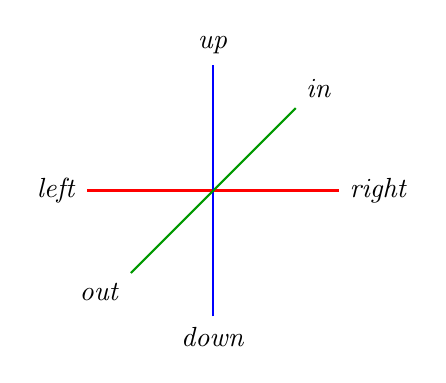
\begin{tikzpicture}[scale=.8]
\draw[thick,red] (-2,0,0) node [black,left] {\textit{left}} -- (2,0,0) node [black,right] {\textit{right}};
\draw[thick,blue] (0,-2,0) node [black,below] {\textit{down}} -- (0,2,0) node [black,above] {\textit{up}};
\draw[thick,green!60!black] (0,0,-3.4) node [black,above right] {\textit{in}} -- (0,0,3.4) node [black,below left] {\textit{out}};
\end{tikzpicture}
\caption{Three-dimensional coordinate frame}\label{fig.frame}
\end{center}
\end{figure}

Rotate the coordinate frame counterclockwise around the $z$-axis, so that the $z$-axis remains unchanged (Figs.~\ref{fig.standard-axis1}-\ref{fig.rotatez}). The new orientation of the frame is (\textit{up}, \textit{left}, \textit{out}). Consider now a rotation of $90^\circ$ around the $x$-axis (Figs.~\ref{fig.standard-axis2}--\ref{fig.rotatex}). This causes the $y$-axis to ``jump out'' of the paper and the $z$-axis to ``fall down'' onto the paper, resulting in the orientation (\textit{right}, \textit{out}, \textit{down}). Finally, consider a rotation of $90^\circ$ around the $y$-axis (Figs.~\ref{fig.standard-axis3}--\ref{fig.rotatey}). The $x$-axis ``drops into'' the paper and the $z$-axis ``falls right'' onto the paper. The new position of the frame is (\textit{in}, \textit{up}, \textit{right}).

\begin{figure}
\subfigures
\begin{minipage}{\textwidth}
\leftfigure{
\begin{tikzpicture}[scale=1.3]
\draw[thick,red,->] (0,0,0) -- (2,0,0) node [black,right] {$x$};
\draw [thick,blue,->] (0,0,0) -- (0,2,0) node [black,above] {$y$};
\draw [thick,green!60!black,->] (0,0,0) -- (0,0,2) node [black,below left] {$z$};
\draw[->] (.5,0,1) arc [start angle=0, end angle=270, radius=3.5mm];
\end{tikzpicture}
}
\hspace{\fill}
\rightfigure{
\begin{tikzpicture}[scale=1.3]
\draw [thick,blue,->] (0,0,0) -- (-2,0,0) node [black,left] {$y$};
\draw [thick,red,->] (0,0,0) -- (0,2,0) node [black,above] {$x$};
\draw [thick,green!60!black,->] (0,0,0) -- (0,0,2) node [black,below left] {$z$};
\end{tikzpicture}
}
\leftcaption{$x$-$y$-$z$ coordinate frame}\label{fig.standard-axis1}
\rightcaption{$x$-$y$-$z$ coordinate frame after rotating $90^\circ$ around the $z$-axis}\label{fig.rotatez}
\end{minipage}
\end{figure}


\begin{figure}
\subfigures
\begin{minipage}{\textwidth}
\leftfigure{
\begin{tikzpicture}[scale=1.3]
\draw [thick,red,->] (0,0,0) -- (2,0,0) node [black,right] {$x$};
\draw [thick,blue,->] (0,0,0) -- (0,2,0) node [black,above] {$y$};
\draw [thick,green!60!black,->] (0,0,0) -- (0,0,2) node [black,below left] {$z$};
\draw[->] (1,.1,0) arc [start angle=0, end angle=270, radius=3.5mm];
\end{tikzpicture}
}
\hspace{\fill}
\rightfigure{
\begin{tikzpicture}[baseline=-4em,scale=1.3]
\draw [thick,red,->] (0,0,0) -- (2,0,0) node [black,right] {$x$};
\draw [thick,green!60!black,->] (0,0,0) -- (0,-2,0) node [black,below] {$z$};
\draw [thick,blue,->] (0,0,0) -- (0,0,2) node [black,below left] {$y$};
\end{tikzpicture}
}
\leftcaption{$x$-$y$-$z$ coordinate frame}\label{fig.standard-axis2}
\rightcaption{$x$-$y$-$z$ coordinate frame after rotating $90^\circ$ around the $x$-axis}\label{fig.rotatex}
\end{minipage}
\end{figure}

\begin{figure}
\subfigures
\begin{minipage}{\textwidth}
\leftfigure{
\begin{tikzpicture}[scale=1.3]
\draw [thick,red,->] (0,0,0) -- (2,0,0) node [black,right] {$x$};
\draw [thick,blue,->] (0,0,0) -- (0,2,0) node [black,above] {$y$};
\draw [thick,green!60!black,->] (0,0,0) -- (0,0,2) node [black,below left] {$z$};
\draw[->] (.3,.8,0) arc [start angle=45, end angle=315, radius=3.5mm];
\end{tikzpicture}
}
\hspace{\fill}
\rightfigure{
\begin{tikzpicture}[baseline=-3.8em,scale=1.3]
\draw [thick,green!60!black,->] (0,0,0) -- (2,0,0) node [black,right] {$z$};
\draw [thick,blue,->] (0,0,0) -- (0,2,0) node [black,above] {$y$};
\draw [thick,red,->] (0,0,0) -- (0,0,-2) node [black,above right] {$x$};
\end{tikzpicture}
}
\leftcaption{$x$-$y$-$z$ coordinate frame}\label{fig.standard-axis3}
\rightcaption{$x$-$y$-$z$ coordinate frame after rotating $90^\circ$ around the $y$-axis}\label{fig.rotatey}
\end{minipage}
\end{figure}

\subsection{The right-hand rule}

There are two orientations for each axis, $2^3=8$ orientations overall. What matters is the relative orientation of one axis with respect to the other two; for example, once the $x$- and $y$-axes have been chosen to lie in the plane of the paper, the $z$-axis can have its positive direction pointing out of the paper or into the paper. The choice must be consistent. The convention in physics and mechanics is the \emph{right-hand rule}\index{right-hand rule}. Curl the fingers of your right hand so that they go from the one axis to another axis. Your thumb now points in the positive direction of the third axis. For the familiar $x$- and $y$-axes on paper, curl your fingers on the path from the $x$-axis to the $y$-axis. When you do so your thumb points out of the paper and this is taken as the positive direction of the $z$-axis. Fig.~\ref{fig.right-hand-rule} shows the right-hand coordinate system displayed with each of the three axes pointing \emph{out of the paper}. According to the right-hand rule the three rotations are:
\begin{quote}
\normalsize
Rotate \emph{from} x \emph{to} y around z,\\
Rotate \emph{from} y \emph{to} z around x,\\
Rotate \emph{from} z \emph{to} x around y.
\end{quote}

\begin{figure}
\begin{center}
\begin{tikzpicture}[scale=.85]
\draw [thick,red,->] (0,0,0) -- (2,0,0) node [black,right] {$x$};
\draw [thick,blue,->] (0,0,0) -- (0,2,0) node [black,above] {$y$};
\draw [thick,green!60!black,->] (0,0,0) -- (0,0,2) node [black,below left] {$z$};
\draw[->] (.5,0,1) arc [start angle=0, end angle=270, radius=3.5mm];
\end{tikzpicture}
\hspace{2em}
\begin{tikzpicture}[scale=.85]
\draw [thick,blue,->] (0,0,0) -- (2,0,0) node [black,right] {$y$};
\draw [thick,green!60!black,->] (0,0,0) -- (0,2,0) node [black,above] {$z$};
\draw [thick,red,->] (0,0,0) -- (0,0,2) node [black,below left] {$x$};
\draw[->] (.5,0,1) arc [start angle=0, end angle=270, radius=3.5mm];
\end{tikzpicture}
\hspace{2em}
\begin{tikzpicture}[scale=.85]
\draw [thick,green!60!black,->] (0,0,0) -- (2,0,0) node [black,right] {$z$};
\draw [thick,red,->] (0,0,0) -- (0,2,0) node [black,above] {$x$};
\draw [thick,blue,->] (0,0,0) -- (0,0,2) node [black,below left] {$y$};
\draw[->] (.5,0,1) arc [start angle=0, end angle=270, radius=3.5mm];
\end{tikzpicture}
\caption{The right-hand rule}\label{fig.right-hand-rule}
\end{center}
\end{figure}

\subsection{Matrices for three-dimensional rotations}
\index{rotation!matrix!three-dimensional}

A three-dimensional rotation matrix is a $3\times 3$ matrix because each point $p$ in a frame has three coordinates $p_x,p_y,p_z$ that must be moved. 
Start with a rotation of $\psi$ around the $z$-axis, followed by a rotation of $\theta$ around the $y$ axis and finally a rotation of $\phi$ around the $x$-axis. For the first rotation around the $z$-axis, the $x$ and $y$ coordinates are rotated as in two dimensions and the $z$ coordinate remains unchanged. Therefore, the matrix is:
\[
\spacearray
R_{z(\psi)}=\left[\begin{array}{ccc}\cos\psi&-\sin\psi&0\\\sin\psi&\cos\psi&0\\0&0&1\end{array}\right]\,.
\]
For the rotation by $\theta$ around the $y$-axis, the $y$ coordinate is unchanged and the $z$ and $x$ coordinates are transformed ``as if'' they were the $x$ and $y$ coordinates of a rotation around the $z$-axis:
\[
\spacearray
R_{y(\theta)}=\left[\begin{array}{ccc}\cos\theta&0&\sin\theta\\0&1&0\\-\sin\theta&0&\cos\theta\\\end{array}\right]\,.
\]
For the rotation by $\phi$ around the $x$-axis, the $x$ coordinate is unchanged and the $y$ and $z$ coordinates are transformed ``as if'' they were the $x$ and $y$ coordinates of a rotation around the $z$-axis:
\[
\spacearray
R_{x(\phi)}=\left[\begin{array}{ccc}1&0&0\\0&\cos\phi&-\sin\phi\\0&\sin\phi&\cos\phi\\\end{array}\right]\,.
\]

It may seem strange that in the matrix for the rotation around the $y$-axis  the signs of the sine function have changed. To convince yourself that matrix for this rotation is correct, redraw the diagram in Fig.~\ref{fig.framea}, substituting $z$ for $x$ and $x$ for $y$ and perform the trigonometric computation.

\subsection{Multiple rotations}

There is a caveat to composing rotations: like matrix multiplication, three\--di\-men\-sion\-al rotations \emph{do not} commute. Let us demonstrate this by a simple sequence of two rotations. Consider a rotation of $90^\circ$ around the $z$-axis, followed by a rotation of $90^\circ$ around the (new position of the) $x$-axis (Fig.~\ref{fig.non-commutative1}). The result can be expressed as (\textit{up}, \textit{out}, \textit{right}).

\begin{figure}
\begin{center}
\begin{tikzpicture}[scale=.85]
\draw [thick,red,->] (0,0,0) -- (2,0,0) node [black,right] {$x$};
\draw [thick,blue,->] (0,0,0) -- (0,2,0) node [black,above] {$y$};
\draw [thick,green!60!black,->] (0,0,0) -- (0,0,2) node [black,below left] {$z$};
\draw[->] (.5,0,1) arc [start angle=0, end angle=270, radius=3.5mm];
\end{tikzpicture}
\hspace{2em}
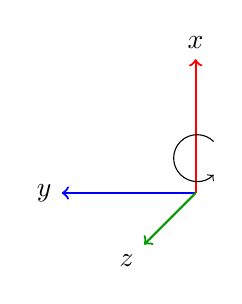
\begin{tikzpicture}[scale=.85]
\draw [thick,blue,->] (0,0,0) -- (-2,0,0) node [black,left] {$y$};
\draw [thick,red,->] (0,0,0) -- (0,2,0) node [black,above] {$x$};
\draw [thick,green!60!black,->] (0,0,0) -- (0,0,2) node [black,below left] {$z$};
\draw[->] (.5,1,.6) arc [start angle=45, end angle=315, radius=3.5mm];
\end{tikzpicture}
\hspace{2em}
\begin{tikzpicture}[scale=.85]
\draw [thick,green!60!black,->] (0,0,0) -- (2,0,0) node [black,right] {$z$};
\draw [thick,red,->] (0,0,0) -- (0,2,0) node [black,above] {$x$};
\draw [thick,blue,->] (0,0,0) -- (0,0,2) node [black,below left] {$y$};
\end{tikzpicture}
\caption{Rotation around the $z$-axis followed by rotation around the $x$-axis}\label{fig.non-commutative1}
\end{center}
\end{figure}

Now consider the commuted operation: a rotation of $90^\circ$ around the $x$-axis, followed by a rotation of $90^\circ$ around the $z$-axis (Fig.~\ref{fig.non-commutative2}). The result can be expressed as (\textit{out}, \textit{left}, \textit{down}), which is not the same as the previous orientation.

\begin{figure}
\begin{center}
\begin{tikzpicture}[scale=.85]
\draw [thick,red,->] (0,0,0) -- (2,0,0) node [black,right] {$x$};
\draw [thick,blue,->] (0,0,0) -- (0,2,0) node [black,above] {$y$};
\draw [thick,green!60!black,->] (0,0,0) -- (0,0,2) node [black,below left] {$z$};
\draw[->] (1.4,.1,0) arc [start angle=0, end angle=270, radius=3.5mm];
\end{tikzpicture}
\hspace{2em}
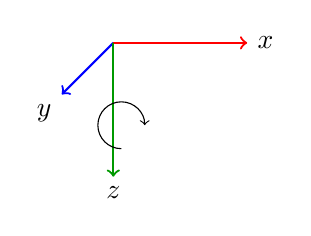
\begin{tikzpicture}[scale=.85,baseline=-3.1em]
\draw [thick,red,->] (0,0,0) -- (2,0,0) node [black,right] {$x$};
\draw [thick,blue,->] (0,0,0) -- (0,0,2) node [black,below left] {$y$};
\draw [thick,green!60!black,->] (0,0,0) -- (0,-2,0) node [black,below] {$z$};
\draw[<-] (.7,-1,.6) arc [start angle=0, end angle=270, radius=3.5mm];
\end{tikzpicture}
\hspace{2em}
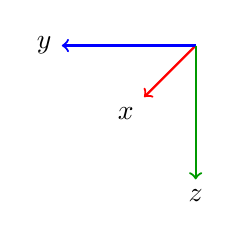
\begin{tikzpicture}[scale=.85,baseline=-3em]
\draw [thick,red,->] (0,0,0) -- (0,0,2) node [black,below left] {$x$};
\draw [thick,blue,->] (0,0,0) -- (-2,0,0) node [black,left] {$y$};
\draw [thick,green!60!black,->] (0,0,0) -- (0,-2,0) node [black,below] {$z$};
\end{tikzpicture}
\caption{Rotation around the $x$-axis followed by rotation around the $z$-axis}\label{fig.non-commutative2}
\end{center}
\end{figure}

\subsection{Euler angles}
\index{Euler angles}

An arbitrary rotation can be obtained by three individual rotations around the three axes, so the matrix for an arbitrary rotation can be obtained by multiplying the matrices for each single rotation. The angles of the rotations are called \emph{Euler angles}. The formulas are somewhat complex and can be found in the references listed at the end of the chapter. Here we demonstrate Euler angles with an example.

\smallskip

\noindent\textbf{Example} Figure~\ref{fig.euler} shows a coordinate frame rotated sequentially $90^\circ$ around the $z$-axis, then the $y$-axis and finally the $x$-axis. This is called a $zyx$ Euler angle rotation. The final orientation is (\textit{in}, \textit{up}, \textit{right}).

\begin{figure}
\begin{center}
\begin{tikzpicture}[scale=.7]
\draw [thick,red,->] (0,0,0) -- (2,0,0) node [black,right] {$x$};
\draw [thick,blue,->] (0,0,0) -- (0,2,0) node [black,above] {$y$};
\draw [thick,green!60!black,->] (0,0,0) -- (0,0,2) node [black,below left] {$z$};
\draw[->] (0,-.3,.1) arc [start angle=0, end angle=270, radius=3mm];
\end{tikzpicture}
\hspace{2em}
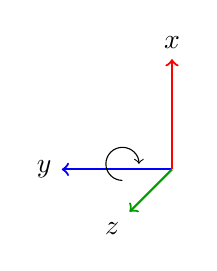
\begin{tikzpicture}[scale=.7]
\draw [thick,blue,->] (0,0,0) -- (-2,0,0) node [black,left] {$y$};
\draw [thick,red,->] (0,0,0) -- (0,2,0) node [black,above] {$x$};
\draw [thick,green!60!black,->] (0,0,0) -- (0,0,2) node [black,below left] {$z$};
\draw[<-] (-.6,.1,0) arc [start angle=0, end angle=270, radius=3mm];
\end{tikzpicture}
\hspace{2em}
\begin{tikzpicture}[scale=.7,baseline=-3em]
\draw [thick,green!60!black,->] (0,0,0) -- (0,2,0) node [black,above] {$z$};
\draw [thick,blue,->] (0,0,0) -- (-2,0,0) node [black,left] {$y$};
\draw [thick,red,->] (0,0,0) -- (0,0,-2.5) node [black,above right] {$x$};
\draw[<-] (.6,.2,-.5) arc [start angle=0, end angle=270, radius=3mm];
\end{tikzpicture}
\hspace{2em}
\begin{tikzpicture}[scale=.7,baseline=-3em]
\draw [thick,blue,->] (0,0,0) -- (0,2,0) node [black,above] {$y$};
\draw [thick,green!60!black,->] (0,0,0) -- (2,0,0) node [black,right] {$z$};
\draw [thick,red,->] (0,0,0) -- (0,0,-2.5) node [black,above right] {$x$};
\end{tikzpicture}
\caption{Euler angles $zyx$ of $(90^\circ,90^\circ,90^\circ)$}\label{fig.euler}
\end{center}
\end{figure}

Let us consider a robotic manipulator that consists of a single joint that can rotate around all three axes. A sequence of rotations is performed as shown in Fig.~\ref{fig.euler}. Consider the point at coordinates $(1,1,1)$ relative to the joint (Fig.~\ref{fig.rotate3}). After the rotations, what are the coordinates of this point in the original fixed frame?

\begin{figure}
\subfigures
\begin{minipage}{\textwidth}
\leftfigure{
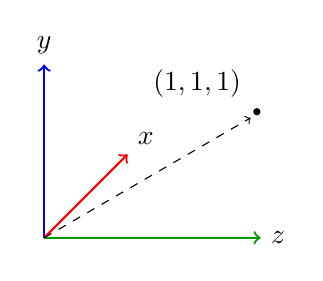
\begin{tikzpicture}[scale=1.1]
\draw [thick,blue,->] (0,0,0) -- (0,2,0) node [black,above] {$y$};
\draw [thick,green!60!black,->] (0,0,0) -- (2.5,0,0) node [black,right] {$z$};
\draw [thick,red,->] (0,0,0) -- (0,0,-2.5) node [black,above right] {$x$};
\draw[->,dashed] (0,0,0) -- (2,1,-1) node[above left,yshift=4pt] {$(1,1,1)$};
\draw[fill] (2,1,-1) circle [xshift=2pt,yshift=2pt,radius=1pt];
\end{tikzpicture}
}
\hspace{\fill}
\rightfigure{
\begin{tikzpicture}[scale=1.1]
\draw [thick,green!60!black,->] (0,0,0) -- (0,2,0) node [black,above] {$z$};
\draw [thick,blue,->] (0,0,0) -- (-2,0,0) node [black,left] {$y$};
\draw [thick,red,->] (0,0,0) -- (0,0,-2.5) node [black,above right] {$x$};
\draw[<-] (.5,.2,-.8) arc [start angle=0, end angle=270, radius=3mm];
\draw[->,dashed] (0,0,0) -- (2,1,-1) node[above left,yshift=4pt] {$(1,-1,1)$};
\draw[fill] (2,1,-1) circle [xshift=2pt,yshift=2pt,radius=1pt];
\end{tikzpicture}
}
\leftcaption{Vector after final rotation}\label{fig.rotate3}
\rightcaption{Vector before rotating around the $x$-axis}\label{fig.rotate2}
\end{minipage}
\end{figure}

This can be computed by leaving the vector fixed and considering the rotations of the coordinate frames. To reach the final position shown in Fig.~\ref{fig.rotate3} the frame was rotated around the $x$-axis from the orientation shown in Fig.~\ref{fig.rotate2}. By examining the figure we see that the coordinates in this frame are $(1,-1,1)$. Proceeding through the previous two frames (Figs.~\ref{fig.rotate1}, \ref{fig.rotate0}), the coordinates are $(1,-1,-1)$ and $(1,1,-1)$.

\begin{figure}
\subfigures
\begin{minipage}{\textwidth}
\leftfigure{
\begin{tikzpicture}[scale=1.1]
\draw [thick,blue,->] (0,0,0) -- (-2,0,0) node [black,left] {$y$};
\draw [thick,red,->] (0,0,0) -- (0,2,0) node [black,above] {$x$};
\draw [thick,green!60!black,->] (0,0,0) -- (0,0,2) node [black,below left] {$z$};
\draw[<-] (-.6,.1,0) arc [start angle=0, end angle=270, radius=3mm];
\draw[->,dashed] (0,0,0) -- (2,1,-1) node[above left,yshift=4pt] {$(1,-1,-1)$};
\draw[fill] (2,1,-1) circle [xshift=2pt,yshift=2pt,radius=1pt];
\end{tikzpicture}
}
\hspace{\fill}
\rightfigure{
\begin{tikzpicture}[scale=1.1]
\draw [thick,red,->] (0,0,0) -- (2.5,0,0) node [black,right] {$x$};
\draw [thick,blue,->] (0,0,0) -- (0,2,0) node [black,above] {$y$};
\draw [thick,green!60!black,->] (0,0,0) -- (0,0,2) node [black,below left] {$z$};
\draw[->] (0,-.3,.1) arc [start angle=0, end angle=270, radius=3mm];
\draw[->,dashed] (0,0,0) -- (2,1,-1) node[above left,yshift=4pt] {$(1,1,-1)$};
\draw[fill] (2,1,-1) circle [xshift=2pt,yshift=2pt,radius=1pt];
\end{tikzpicture}
}
\leftcaption{Vector before rotating around the $y$-axis}\label{fig.rotate1}
\rightcaption{Vector in the fixed frame before rotating around the $z$-axis}\label{fig.rotate0}
\end{minipage}
\end{figure}

These coordinates can be computed from the rotation matrices for the rotations around the three axes. The coordinates of the final coordinate frame are $(1,1,1)$, so in the frame before the rotation around the $x$-axis the coordinates were:
\[
\spacearray
\left[\begin{array}{ccc}1&0&0\\0&0&-1\\0&1&0\\\end{array}\right]
\left[\begin{array}{c}1\\1\\1\end{array}\right]=
\left[\begin{array}{c}1\\-1\\1\end{array}\right]\,.
\]
The coordinates in the frame before the rotation around the $y$-axis were:
\[
\spacearray
\left[\begin{array}{ccc}0&0&1\\0&1&0\\-1&0&0\\\end{array}\right]
\left[\begin{array}{c}1\\-1\\1\end{array}\right]=
\left[\begin{array}{c}1\\-1\\-1\end{array}\right]\,.
\]
Finally, the coordinates in the fixed frame before the rotation around the $z$-axis were:
\[
\spacearray
\left[\begin{array}{ccc}0&-1&0\\1&0&0\\0&0&1\\\end{array}\right]
\left[\begin{array}{c}1\\-1\\-1\end{array}\right]=
\left[\begin{array}{c}1\\1\\-1\end{array}\right]\,.
\]

For three arbitrary $zyx$ Euler angle rotations: $\psi$ around the $z$-axis, then $\theta$ around the $y$-axis and finally $\phi$ around the $x$-axis the rotation matrix is:
\[
R=R_{z(\psi)}R_{y(\theta)}R_{x(\phi)}\,.
\]
It may seem strange that the order of the matrix multiplication (which is always from right to left) is opposite the order of the rotations. This is because we are taking a vector in the final coordinate frame and transforming it back into the fixed frame to determine its coordinates in the fixed frame.

\begin{framed}
\act{Multiple Euler angles}{euler-multiple}
\begin{itemize}
\item Multiply the three matrices to obtain a single matrix that directly transforms the coordinates from $(1,1,1)$ to $(1,1,-1)$.
\item Perform the same computation for other rotations, changing the sequence of the axes and the angles of rotation.
\end{itemize}
\end{framed}

\subsection{The number of distinct Euler angle rotations}
\index{Euler angles!number of}

There are three axes so there should be $3^3=27$ sequences of Euler angles. However, there is no point in rotating around the same axis twice in succession because the same result can be obtained by rotating once by the sum of the angles, so there are only $3\cdot 2\cdot 2=12$ different Euler angles sequences.  The following activity asks you to explore different Euler angle sequences.

\begin{framed}
\act{Distinct Euler angles}{euler-distinct}
\begin{itemize}
\item To experiment with three-dimensional rotations, it is helpful to construct a coordinate frame from three mutually perpendicular pencils or straws.
\item Draw the coordinate frames for a $zyz$ Euler angle rotation, where each rotation is by $90^\circ$. %Answer: $(l,o,u)$
\item What $zyz$ rotation gives the same result at the $zyx$ rotation shown in Fig.~\ref{fig.euler}? %Answer: $(0,90,0)$
\item Experiment with other rotation sequences and with angles other than $90^\circ$.
\end{itemize}
\end{framed}

\section{Advanced topics in three-dimensional transforms}\label{s.advanced-three}
\index{rotation!three-dimensional}

Now that you have tasted three-dimensional rotations, we survey the next steps in learning this topic which you can study in the textbooks listed in the references.

There are $12$ Euler angles and the choice of which to use depends on the intended application. Furthermore, there is a different way of defining rotations. Euler angles are \emph{moving axes} transforms, that is, each rotation is around the \emph{new} position of the axis after the previous rotation. In Fig.~\ref{fig.euler}, the second rotation is around the $y$-axis that now points left, not around the original $y$-axis that points up. It is also possible to define \emph{fixed axes} rotations in which subsequent rotations are around the original axes of the coordinate system. In three dimensions, homogeneous transforms that include translations in addition to rotations can be efficiently represented as $4\times 4$ matrices.

Euler angles are relatively inefficient to compute and suffer from computational instabilities. These can be overcome by using \emph{quaternions}\index{quaternions}, which are a generalization of complex numbers. Quaternions use three ``imaginary'' numbers $i,j,k$, where:
\[
i^2 = j^2 = k^2 = ij\,k = -1\,.
\]
Recall that a vector in the two-dimensional plane can be expressed as a complex number $x+\vec{i}\,y$. Rotating the vector by an angle $\theta$ can be performed by multiplying by the value $\cos \theta + \vec{i} \sin \theta$.  Similarly, in three dimensions, a vector can be expressed as a \emph{pure quaternion} with a zero real component: $p=0+x\,\vec{i} + y\,\vec{j} + z\,\vec{k}$. Given an axis and an angle, there exists a quaternion $q$ that rotates the vector around the axis by this angle using the formula $qpq^{-1}$. This computation is more efficient and robust than the equivalent computation with Euler angles and is used in a variety of contexts such as aircraft control and computer graphics.


\section{Summary}

Kinematics is the description of the motion of a robot. In forward kinematics, we are given a set of commands for the robot and we need to compute its final position relative to its initial position. In inverse kinematics, we are given a desired final position and need to compute the commands that will bring the robot to that position. This chapter has demonstrated kinematic computations for a simple two-dimensional robotic manipulator arm. In practice, manipulators move in three-dimensions and the computations are more difficult. Exact solutions for computing inverse kinematics usually cannot be found and approximate numerical solutions are used.

There are many ways of defining and computing arbitrary rotations. We mentioned the Euler angles where an arbitrary rotation is obtained by a sequence of three rotations around the coordinate axes. Quaternions, a generalization of complex numbers, are often used in practice because they are computationally more efficient and robust.

\section{Further reading}

Advanced textbooks on robotic kinematics and related topics are those by Craig \cite{craig} and Spong et al. \cite{spong}. See also Chapter~3 of Correll \cite{correll}. Appendix~B of \cite{craig} contains the rotation matrices for all the Euler angle sequences. The video lectures by Angela Sodemann are very helpful:\\
\url{https://www.youtube.com/user/asodemann3},\\
\url{http://www.robogrok.com/Flowchart.html}.

Although not a book on robotics, Vince's monograph on quaternions \cite{vince} gives an excellent presentation of the mathematics of rotations.

\bibliographystyle{spmpsci}
\bibliography{er}
